\documentclass[a4paper,12pt]{article}
\usepackage{amsmath,amssymb,amsfonts,amsthm}
\usepackage{tikz}
\usepackage[utf8x]{inputenc}
\usepackage[T2A]{fontenc} 
\usepackage[russian]{babel}
\usepackage{cmap} 
\usepackage{ gensymb }
% Так ссылки в PDF будут активны
\usepackage[unicode]{hyperref}
\usepackage{ textcomp }
\usepackage{indentfirst}
\usepackage[version=3]{mhchem}

% вы сможете вставлять картинки командой \includegraphics[width=0.7\textwidth]{ИМЯ ФАЙЛА}
% получается подключать, как минимум, файлы .pdf, .jpg, .png.
\usepackage{graphicx}
% Если вы хотите явно указать поля:
\usepackage[margin=1in]{geometry}
% Или если вы хотите задать поля менее явно (чем больше DIV, тем больше места под текст):
% \usepackage[DIV=10]{typearea}

\usepackage{fancyhdr}

\newcommand{\bbR}{\mathbb R}%теперь вместо длинной команды \mathbb R (множество вещественных чисел) можно писать короткую запись \bbR. Вместо \bbR вы можете вписать любую строчку букв, которая начинается с '\'.
\newcommand{\eps}{\varepsilon}
\newcommand{\bbN}{\mathbb N}
\newcommand{\dif}{\mathrm{d}}

\newtheorem{Def}{Определение}


\pagestyle{fancy}
\makeatletter % сделать "@" "буквой", а не "спецсимволом" - можно использовать "служебные" команды, содержащие @ в названии
\fancyhead[L]{\footnotesize Лабораторные работы по общей физике}%Это будет написано вверху страницы слева
\fancyhead[R]{\footnotesize ФУПМ МФТИ}
\fancyfoot[L]{\footnotesize \@author}%имя автора будет написано внизу страницы слева
\fancyfoot[R]{\thepage}%номер страницы —- внизу справа
\fancyfoot[C]{}%по центру внизу страницы пусто

\renewcommand{\maketitle}{%
	\noindent{\bfseries\scshape\large\@title\ \mdseries\upshape}\par
	\noindent {\large\itshape\@author}
	\vskip 2ex}
\makeatother
\def\dd#1#2{\frac{\partial#1}{\partial#2}}


\title{10.1. Электронный парамагнитный резонанс}
\author{Хурсик Екатерина} 
\date{\today}

\begin{document}
	
\maketitle
\section*{Цель работы}
1)Исследовать электронный парамагнитный резонанс в молекуле ДФПГ;
2)определить $g$-фактор электрона; 3)измерить ширину линии.
\section{Теоретическое введение}
\subsection*{g-фактор}
Энергетический уровень электрона в присутствии магнитного поля $B$ расщепляется на два подуровня, расстояние между которыми равно:
\begin{equation}
    \Delta E = E_2 - E_1 = 2\mu B
\end{equation}
Между этими двумя уровнями возможны переходы. Они могут возбуждаться внешним высокочастотным магнитным полем подходящих характеристик.
Резонансное значение частоты определяется из очевидного соотношения:
\begin{equation}
    \hbar\omega_0 = \Delta E =2\mu B
\end{equation}
    
В работе требуется получить ЭПР сигнал на ДФПГ. Известно, что связь между магнитным моментом электрона и его механическим моментом выражается через гиромагнитное соотношение:
\begin{equation}
    \bf{\mu} = \gamma\bf{M}
\end{equation}
Если магнитный момент выражается в магнетонах Бора, а механический в единицах $\hbar$, то связь выражается через фактор Ланде:
\begin{equation}
    \frac{\bf{\mu}}{\mu_\text{Б}} = \frac{g\bf{M}}{\hbar}
\end{equation}
Эта формула справедлива и для проекций. Можно выразить $g$-фактор через определяемые экспериментально величины:
\begin{equation}
    g = \frac{\hbar\omega_0}{\mu_\text{Б} B_0},
\end{equation}
где $\mu_\text{Б}$ -- магнетон Бора, а величину магнитного поля $B_0$ можно рассчитать из соотношения
\begin{equation*}
    V_\Pi=NB_0S\omega_\simeq,
\end{equation*} 
где $\omega_\simeq=2\pi\nu$ - угловая частота переменного тока ($\nu$-частота сети).
\subsection*{Ширина линии ЭПР}
Для определения ширины линии ЭПР определяем по экрану осциллографа полный размах
модулирующего поля (в делениях шкалы) $A_\text{полн}$ и полную ширину кривой резонансного
поглощения на полувысоте $A_{1/2}$ . Берём пробную катушку и
вносим её внутрь соленоида максимально близко к образцу. Переменное поле
модуляционных катушек наводит в пробной катушке ЭДС индукции, по которой можно
определить величину поля. Параметры пробной катушки указаны на ней ($N_{проб} = 46$,
$d = 14.6 \pm 0.1 \; \text{мм}$ и ЭДC $\varepsilon_i=2,51\cdot 10^{-3} B$).
Вольтметр измеряет действующее значение ЭДС индукции, а полный размах
сигнала на экране осциллографа соответствует амплитудному значению переменного поля.
По измеренной ЭДС индукции $\varepsilon_i$ и параметрам катушки (числу витков $N_\text{проб}$ и диаметру
намотки $d$) определите амплитуду модулирующего поля $B_\text{мод} = \sqrt{2}\frac{2\varepsilon_i}{\pi^2 d^2N_\text{проб} \nu}$,
где $\nu$ - частота модулирующего напряжения. Полуширина на полувысоте линии резонансного
поглощения (в единицах поля) может быть тогда получена как $\Delta B=\frac{A_{1/2}}{A_\text{полн}}B_\text{мод}$\,.
\subsection*{Установка}
Для исследования электронного парамагнитного резонанса в данной работе используется
радиоспектроскоп. Его действие основано на уменьшении добротности контура при
появлении резонансных парамагнитных потерь.
Величина постоянного магнитного поля $B$, резонансная частота колебательного
контура и частота генератора $\omega$ выбираются так, чтобы они были близки к
значениям, удовлетворяющим уравнению $\hbar\omega_0=\Delta E=2\mu B$.

При наступлении ЭПР поглощение энергии в образце увеличивается, добротность
колебательного контура падает, и амплитуда колебаний в контуре уменьшается.

Схема спектроскопа приведена на рисунке:

\begin{figure}[h!]
    \begin{center}
        \begin{minipage}{0.49\linewidth}
            \centering
            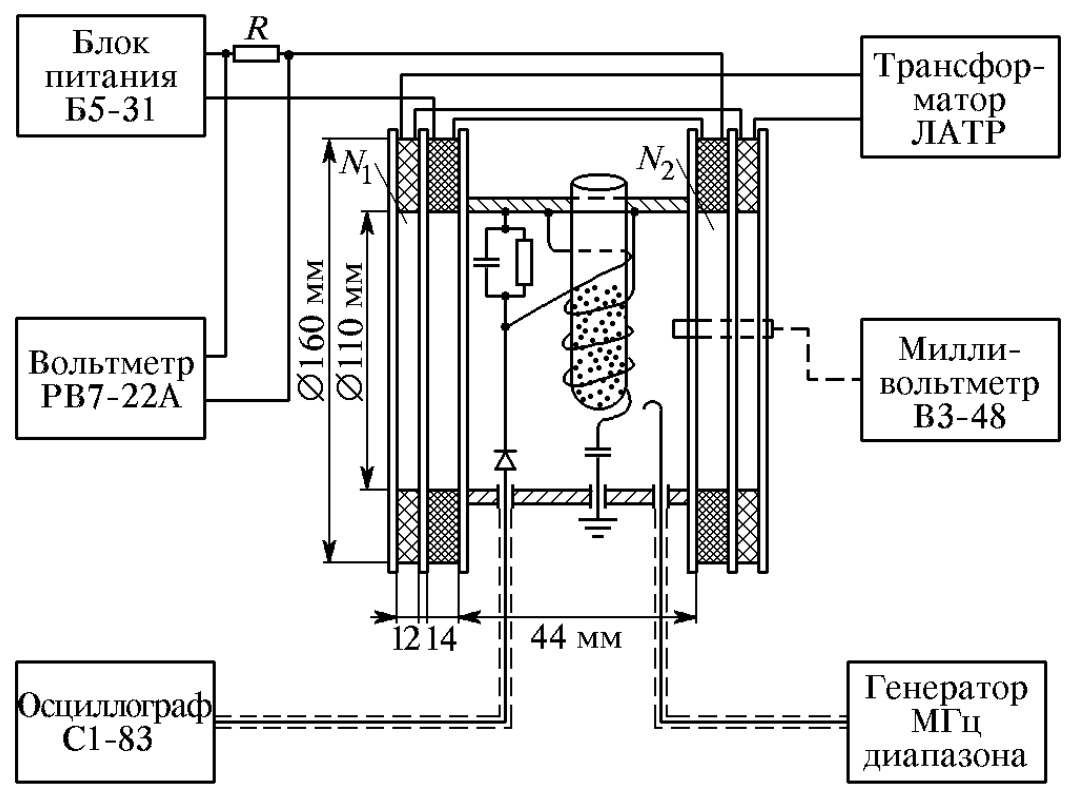
\includegraphics[width=0.9\linewidth]{exp.png}
            \caption{Схема установки}
        \end{minipage}
    \end{center}
\end{figure}        
    
Параметры установки: $N_1 = 1500, d_1 = 0.23\,cm, N_2 = 4500, d_2=0.29\,cm$
\section{Метод достижения цели}
\subsection{}
Для наблюдения электронного парамагнитного резонанса нужно поместить 
исследуемое вещество в магнитное поле и измерить поглощение электромагнитного
излучения, частота которого уловлетворяет соотношению (2).\\
При наступлении ЭПР поглощение энергии в образце увеличивается, добротность
колебательного контура падает, а соответственно амплитуда колебаний в контуре уменьшается.
\subsection{}
Измеряем $g$-фактор, для чего находим резонансное значение частоты $\omega_0$ и индукции $B_0$.
Резонансную частоту $\omega_0$ определяем по лимбу генератора.\\
Величину магнитного поля $B_0$ поля измеряем следующим способом:
\begin{itemize}
    \item помещаем пробную катушку внутрь основных катушек;
    \item снимаем показания лампового милливольтметра $V$;
    \item зная параметры пробной катушки из соотношения $V=NB_0S\omega_\simeq$, где $\omega_\simeq$ - угловая частота переменного тока, определяем величину магнитного поля $B_0$;
    \item вычисляем $g$-фактор по формуле $g=\frac{\hbar\omega_0}{\mu_\text{Б}B_0}$.
\end{itemize}
\subsection{}
Измерение ширины линии производится по экрану осциллографа.\\
Получив сигнал ЭПР, переключаем осциллограф в режим временной развёртки
на развёртку от модуляционных катушек. Длина развёртки есть удвоенная
амплитуда модулирующего поля. Амплитуду этого поля определяем при помощи
милливольтметра и пробной катушки.\\
Ширину линии получаем, пользуясь формулой (2).

\section{Ход работы}

Настроим генератор на резонансную частоту колебательного контура,
определили значение частоты при максимальном и половинных
значениях амплитуды выведенного на осциллограф сигнала:

$\omega_{0} = 125.76 \, \text{МГц}$,

$\omega_{h} = 126.94 \, \text{МГц}$,

$\omega_{l} = 126.46 \, \text{МГц}$.\\
Рассчитаем добротность
\begin{equation*}
    Q = \frac{\omega_0}{\Delta\omega} = \frac{125.76}{0.48} = 262
\end{equation*}
\newpage
Теперь настроим установку на наблюдение резонансного сигнала.
Резонансное поглощение возникает при совпадении в некоторые моменты времени поля $B(t)$ с полем резонансного поглощения на частоте колебательного контура $B_0=\frac{\mathrm{h}f_0}{g\mu_B}$.

\begin{figure}[h!]
    \begin{center}
        \begin{minipage}{0.49\linewidth}
            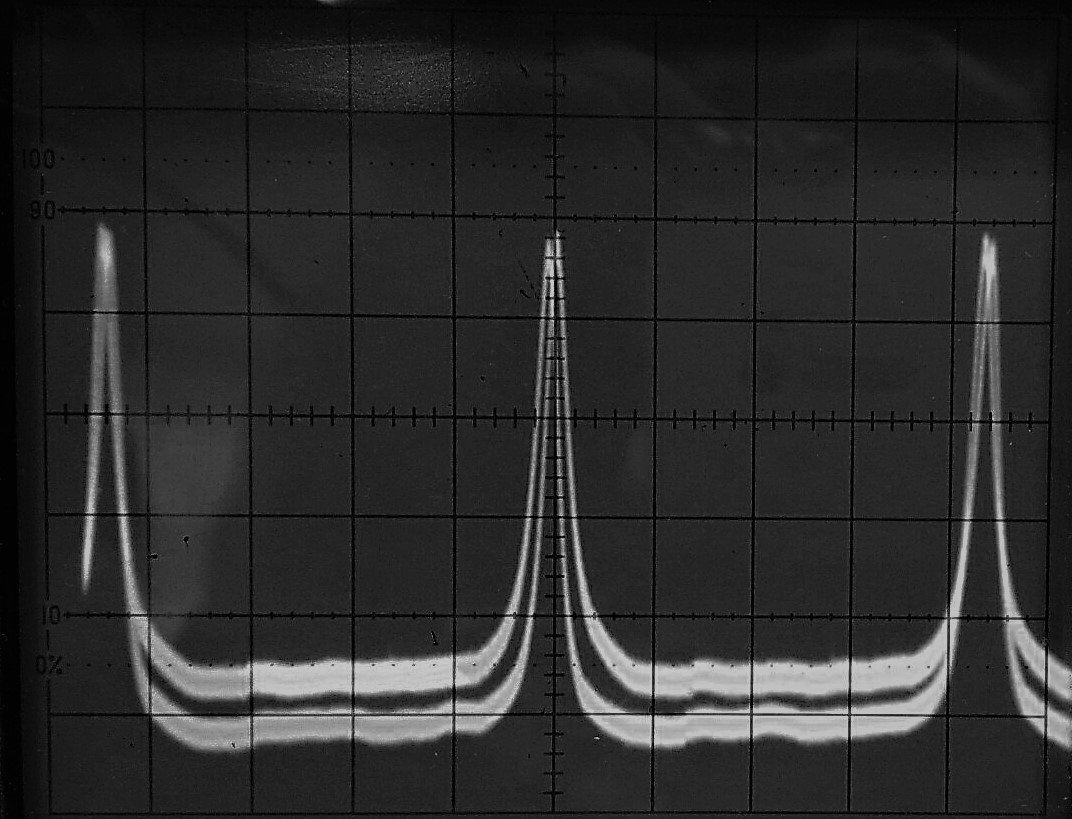
\includegraphics[width=\linewidth]{oscilloscope.jpg}
            \caption{Резонансное поглощение}
        \end{minipage}
        \hfill
        \begin{minipage}{0.49\linewidth}
            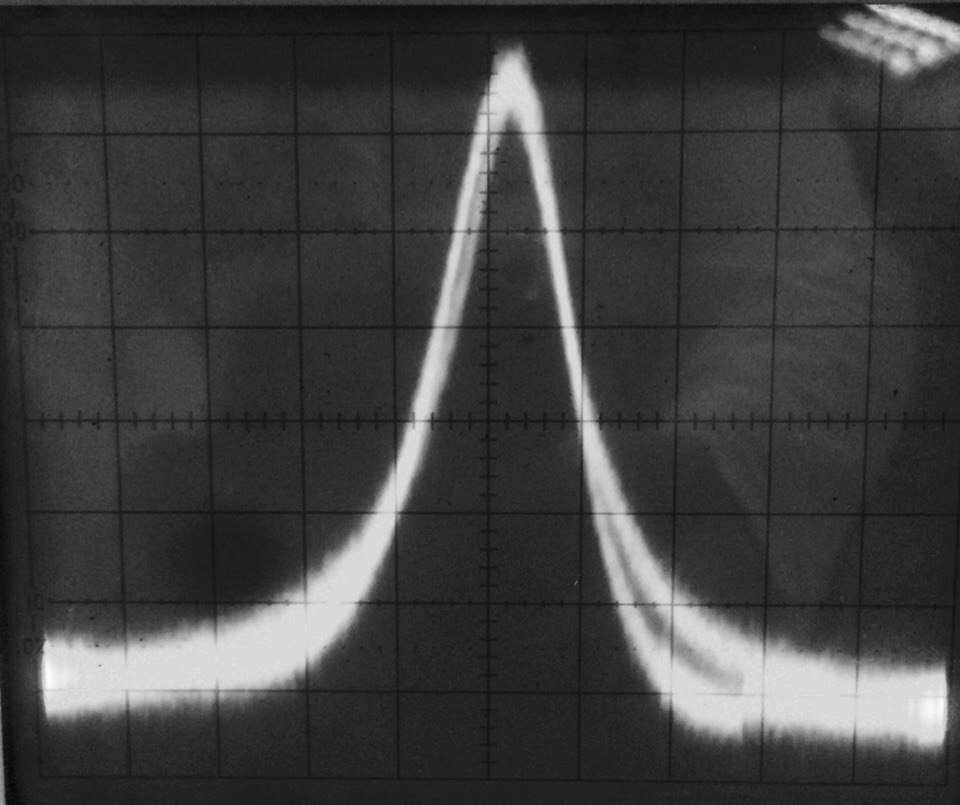
\includegraphics[width=\linewidth]{second.jpg}
            \caption{Точно настроенный пик}
        \end{minipage}
    \end{center}
\end{figure}    
Переменное поле модуляционных катушек наводит в пробной катушке ЭДС индукции,
по которой можно определить величину поля. 
Зная параметры катушки $N_{проб} = 46$, $d = 14.6 \pm 0.1 \; \text{мм}$ и ЭДC $\varepsilon_i=2,51\cdot 10^{-3} B$ , определим величину модулирующего поля:
\begin{equation*}
    B_\text{мод} = \sqrt{2} \frac{2\varepsilon_i}{\pi^2 d^2N_{проб} \nu} = \sqrt{2} \frac{2 \cdot 2.51 \cdot 10^{-3}\, \text{В}}{\pi^2 \cdot 14.6^2 \cdot 10^{-6} \, \text{м} \cdot 46  \cdot 50\, \text{Гц}}  = 1.47 \cdot 10^{-3} \,\text{Тл} = 1.47 \, \text{мТл}
\end{equation*}
Рассчитаем погрешность измерения $B_\text{мод}$.
\begin{equation*}
    \varepsilon_{B_\text{мод}}=\varepsilon_d=0,7\%\quad\rightarrow\quad B_\text{мод}=(1,47\pm0,01)\,\text{мТл}
\end{equation*}
Тогда для полуширины на полувысоте линии резонансного поглощения (в единицах поля) получим
\begin{equation}
    \Delta B  = \frac{A_{1/2}}{A_{\text{полн}}} B_{\text{мод}} = \frac{1}{10.4}\cdot 1.47 \,\text{мТл} = 0.14 \,\text{мТл}  
\end{equation}
\newpage
Определяем g-фактор. Для этого подаем в основные катушки переменный ток,
а ЭДС индукции измеряем при помощи пробной катушки. Строим каллибровочный график:

\begin{figure}[h!]
    \begin{center}
        \begin{minipage}{0.75\linewidth}
            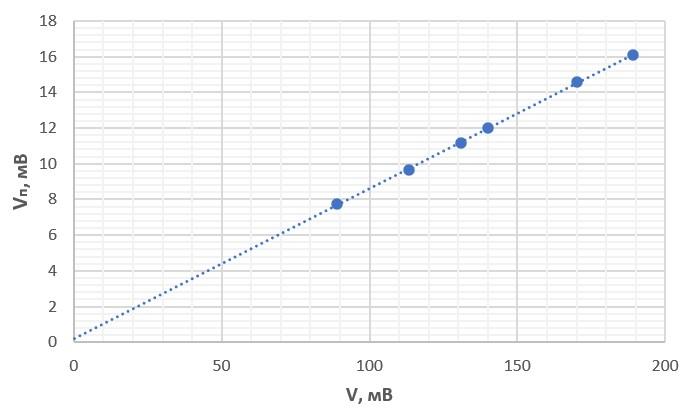
\includegraphics[width=\linewidth]{cal.jpg}
            \caption{Зависимость ЭДC индукции в пробной катушке от падения напряжения в цепи основных катушек}
        \end{minipage}
        \hfill
        \begin{minipage}{0.21\linewidth}
            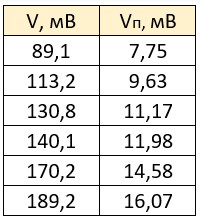
\includegraphics[width=\linewidth]{2020-10-11.jpg}
        \end{minipage}
    \end{center}
\end{figure} 
Найдём зависимость ЭДC индукции в пробной катушке от падения напряжения на резисторе в цепи основных катушек.

Определим по графику тангентс угла наклона:
\begin{equation*}
    \quad\tg\alpha=k=0,086.
\end{equation*}
При $V = 122.84\,\mathrm{mV}$ получаем $V_\Pi = 10.56 \,\text{мВ}$.

Определим погрешность измерений $V_\Pi$.\\
Погрешность измерений $V_\Pi$ есть случайная погрешность, она же средняя квадратичная.
Вычисляем её по формуле
\begin{equation*}
    <\sigma(V_\Pi)>=\sqrt{\frac{1}{n(n-1)}\sum\limits_{i=1}^n(V_{\Pi_i}-<V_\Pi>)^2}=\sqrt{\frac{1}{6\cdot5}\sum\limits_{i=1}^n(V_{\Pi_i}-10,56)^2}=0,04.
\end{equation*}
\begin{figure}[h!]
    \begin{center}
        \begin{minipage}{0.75\linewidth}
            \centering
            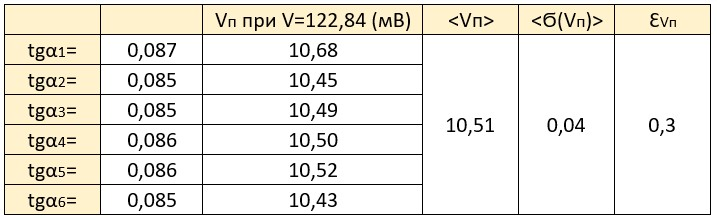
\includegraphics[width=\linewidth]{2020-10-12.jpg}
            \caption{Расчёт погрешности}
        \end{minipage}
    \end{center}
\end{figure}

Теперь можем записать: $\quad V_\Pi=(10,56\pm0,04) \,\text{мВ}, \, \varepsilon=0,3\%$.\\
Рассчитаем величину магнитного поля $B_0$.
\begin{equation*}
    B_0=\frac{2V_\Pi}{N\pi^2d^2\nu}=\frac{2\cdot10,56\cdot10^{-3}}{46\cdot3,14^2\cdot14,6^2\cdot10^{-6}\cdot50}=4,37 \,\text{мВ}
\end{equation*}
Рассчитаем погрешность измерений $B_0$.
\begin{equation*}
    \varepsilon_d=\frac{0,1}{14,6}\cdot100\%=0,7\%,\,\varepsilon_{V_\Pi}=0,3\%\quad\rightarrow\quad \varepsilon_{B_0}=\sqrt{2{\varepsilon_d}^2+{\varepsilon_{V_\Pi}}^2}=1\%.
\end{equation*}
Итого получаем $B_0=(4,37\pm0,04)\,\text{мВ}$.\\

Рассчитаем $g$-фактор.
\begin{equation*}
    g=\frac{\hbar\omega_0}{\mu_\text{Б}B_0}=\frac{6,63\cdot10^{-34}\cdot125,76\cdot10^6}{9,27\cdot10^{-24}\cdot4,37\cdot10^{-3}}=2,06
\end{equation*}
Рассчитаем погрешность вычисления $g$-фактора:
\begin{equation*}
    \varepsilon_g=\varepsilon_{B_0}=1\%\quad\rightarrow\quad g=2,06\pm0,02
\end{equation*}
\section{Вывод}

Рассчитали $g-$фактор, а также проверили достоверность полученных результатов в определении
$g$-фактора и ширины линии ЭПР в кристаллическом ДФПГ.
    
\end{document}
